\chapter{Introduction}

The existence of additional $U(1)$ gauge symmetries of nature are common in
several Beyond the Standard Model (BSM) theories \cite{goodsell2010, 
candelas1985, andreas2013, jaeckel2010}. Such theories envision the associated
gauge boson ($A'$, ``dark'', ``hidden'', ``heavy'' photon) inhabiting a 
``hidden sector''
consisting of a complex of particles and gauge bosons.  Probing the 
structure of such a hidden sector may be possible through several different portals
including ``kinetic mixing''.  In fact, it is natural for the $A'$ to 
kinematically mix with the Standard Model (SM) photon through the interaction
of massive fields carrying both SM hypercharge and dark charge \cite{holdom1986}.
The mixing of the photon with the $A'$ would not only allow searching for
new hidden sector particles, but also dark matter which some theoretical models
have envisioned as inhabiting the hidden sector, with it's interactions mediated
via an $A'$ \cite{arkani-hamed2009, pospelov2009, cheung2009, arkani-hamed2008}.

The chapter that follows will motivate the need to search for an $A'$.  
This will include an overview of current astrophysical anomalies
that may be explained assuming a dark matter candidate that couples to a 
heavy photon.  Finally, a review of current experimental limits on the $A'$ 
coupling strength will be given.

\section{Theoretical Formalism and Physics Motivation}

As Holdom \cite{holdom1986} realized in the mid eighties, in a theory with 
$U(1)_Y \times U(1)'$, there is a term in the gauge part of the Lagrangian 
that allows $U(1)_Y$ and $U(1)'$ to mix.  The gauge part of such a theory can
be written as
\begin{equation}
    \mathcal{L}_{\text{gauge}} = - \frac{1}{4} F_Y^{\mu \nu}F_{Y, \mu \nu}
                          - \frac{1}{4} F'^{\mu \nu}F'_{\mu \nu}
                          + \frac{1}{2} \epsilon F'^{\mu \nu} F_{Y, \mu \nu}
    \label{eqn:l_gauge}
\end{equation}
%the associated gauge boson (heavy photon,
%dark photon or $A'$) can couple to the SM photon through the ``kinetic mixing''
%interaction
where $F'_{\mu \nu} = \partial_{\mu}A'_{\nu} - \partial_{\nu}A'_{\mu}$ 
($F^{\mu \nu}_{Y} = \partial^{\mu}A^{\nu} - \partial^{\nu}A^{\mu}$) is the
field strength tensor of the heavy photon (SM hypercharge) and $\epsilon$ is a
dimensionless coupling constant.  Illuminating the low-energy effects that result
from kinetic mixing can be achieved by decoupling the gauge fields through the
redefinition of the SM hypercharge gauge field as
\begin{equation}
    A_{\mu} \rightarrow A_{\mu} - \epsilon A'_{\mu}.
\end{equation}
Ignoring all $\epsilon^2$ terms that arise from such a transformation, this
results in the diagnolization of \ref{eqn:l_gauge} as
\begin{equation}
    \mathcal{L}_{\text{gauge}} = - \frac{1}{4} F_Y^{\mu \nu}F_{Y, \mu \nu}
                          - \frac{1}{4} F'^{\mu \nu}F'_{\mu \nu}.
\end{equation}
However, the redefinition of the field also affects the interaction term of 
the Lagrangian, $\mathcal{L}_{int} = A^{\mu}J_{\mu}^{EM}$ as
\begin{equation}
    A^{\mu}J_{\mu}^{EM} \rightarrow (A^{\mu} - \epsilon A'^{\mu})J_{\mu}^{EM}.
\end{equation}
As a result, an effective coupling is induced between the electromagnetic current and 
the heavy photon field that is suppressed by a factor of $\epsilon$.

Mixing between the SM photon and the heavy photon can naturally be 
generated at one-loop assuming there exists heavy states, ($\Phi$, $\Phi'$), 
that are charged under both the SM hypercharge and dark charge (see Fig. \ref{fig:ap_loop}).
\begin{figure}
    \centering
    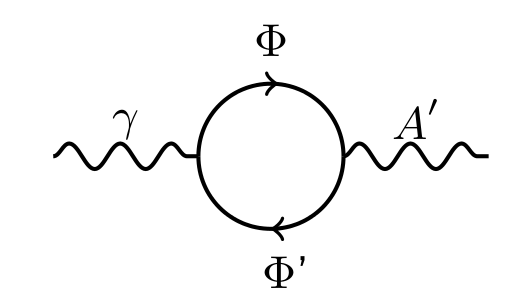
\includegraphics[width=0.5\textwidth]{images/aprime_loop.png}
    \caption{Kinetic mixing of a Standard Model photon with a heavy photon 
    at one-loop through the interaction of massive fields.}
    \label{fig:ap_loop}
\end{figure}
This generates values of $\epsilon$ on the order of 
\begin{equation}
    \epsilon \sim \frac{g_Yg_D}{16\pi^2}\ln\left(\frac{m_{\Phi}}{m_{\Phi'}} \right)
             \sim 10^{-3} - 10^{-1} 
\end{equation}
where $g_Y$ ($g_D$) are the SM hypercharge (dark) coupling and 
$(m_{\Phi}, m_{\Phi'})$ are the masses of the two particles
\cite{arkani-hamed2008, Bjorken:2009mm}.  In some string theory constructions, 
values as small as $\epsilon \sim 10^{-12}$ are expected 
\cite{goodsell2010,Goodsell:2009xc, Cicoli:2011yh}.

%
% If I have time, I need to add a paragraph explaining how an A' would acquire
% mass.
%

The possibility that a new gauge boson can couple to charged SM particles is 
very appealing.  It may offer one of the few portals to probe a new sector 
composed of light weakly coupled particles and possibly dark matter
(see section 1.2).  Such a coupling can be exploited by current and future
experimental programs in order to measure the properties of
the hidden sector and possible provide insight into may outstanding physics puzzles.

\section{Motivations for a Heavy Photon from Dark Matter}

Although the existence of dark matter (DM) has been firmly established through its
gravitational interaction \cite{popolo2014}, its exact nature continues to elude
us. An appealing
possibility is that DM inhabits a ``hidden sector'' with it's interactions 
mediated by an $A'$.  In turn, the kinetic mixing of the $A'$ with the SM 
photon may provide a portal that would allow the exploration of not only the 
properties of DM but the hidden sector itself.  Furthermore, several recently
observed astrophysical anomalies \cite{pamela2008, ackermann2012, aguilar2013, 
hooper2011, linden2011, abazajian2012, hooper2013, Bulbul:2014sua}
may have a dark matter interpretation if it's
charge under an $A'$.  A summary of those anomalies along with their dark matter
interpretation will be presented here.

\subsection{Cosmic Rays}

Interest in hidden sector models surged in 2008 with the announcement by 
The Payload for Antimatter Matter Exploration and Light-nuclei Astrophysics \\ 
(PAMELA) of an unforeseen rise in the ratio of the cosmic ray (CR) positron flux
to CR electron flux, $e^{+}/(e^{+} + e^{-})$, above 10 GeV \cite{pamela2008}.
The rise was later confirmed by both the 
Fermi Gamma-Ray Space Telescope \cite{ackermann2012} and Alpha Magnetic 
Spectrometer-02 (AMS-02) \cite{aguilar2013} experiments and observed to continue
up to 200 GeV. 

The main source of CR positrons 
was expected to come from the interaction of CR nuclei with the interstellar 
medium (secondary production).  If such a production mechanism was dominant, 
cosmic ray propagation models predicted the fraction would fall with increasing
energy.  The observed rise lead to the speculation of additional sources of 
positrons including pulsars\cite{yin2013, linden2013}.

One attractive scenario that could account for the rise was the annihilation of
DM.  In particular, models where DM annihilates to leptons ($e^+e^-, \mu^+\mu^-$)
where found to fit the data fairly well.  However, such models require much 
larger annihilation rates than those that would produce the observed
DM relic density \cite{cholis2009}. Alternatively, if DM annihilates
to a heavy photon which subsequently decays to $e^{+}e^{-}$ 
(Fig. \ref{fig:dm_annihilation}), an enhancement in
\begin{figure}[t]
    \centering
    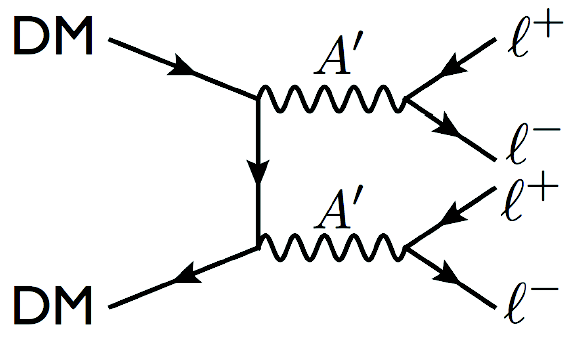
\includegraphics[width=0.5\textwidth]{images/dm_annihilation.png}
    \caption{Dark matter annihilation to a heavy photon which subsequently 
             decays into a pair of leptons.}
    \label{fig:dm_annihilation}
\end{figure}
the annihilation cross-section of DM at low velocities can be achieved through
the Sommerfeld effect \cite{arkani-hamed2009}.  In such a scenario, the annihilation 
cross-section that leads to the currently observed relic abundance would remain
unaffected since the velocity of DM in the early universe was high. 

%The most recent observations by AMS-02 seem to favor 
%This model became less favorable as higher
%precision measurements of the positron flux became available.  In fact, 
%recent measurements of the cosmic microwave background (CMB) have put very 
%tight constraints on such a scenario.

\subsection{Light Dark Matter}

Recently, an analysis of three years of data collected by the Fermi Large Area
Telescope observed an extended emission in the spectrum of gamma-rays 
originating from the Galactic Center 
\cite{hooper2011, linden2011, abazajian2012, hooper2013}.  Several models have been 
devised to try to explain the emission including the collision of energetic 
protons accelerated by a super-massive black hole \cite{Hooper:2010mq}, 
pulsars \cite{Abazajian:2010zy} and dark matter annihilation to leptons or 
hadron \cite{Hooper:2010mq, Goodenough:2009gk}.  The emission can also
be explained in the context of dark matter annihilating to an $A'$ which 
subsequently decays to SM particles \cite{Hooper:2012cw}.  Such a model assumes
a dark matter candidate of mass $\sim$ 10 GeV decaying to a heavy photon
with a mass $\sim$ 100 MeV. 

Another anomaly that can be explained in the context of a light dark matter
candidate that couples to a heavy photon is the observance
of a 3.5 keV line from a cluster of galaxies \cite{Bulbul:2014sua}.  In this case, 
dark matter is assumed to self-interact via an $A'$ producing an excited state.
The excited state then decays and, in the case where 
$m_{\chi^*} - m_{\chi} < 2m_e$, produces an X-ray line 
\cite{Finkbeiner:2014sja}.

\section{Current Limits on Heavy Photons}

\subsection{Electron Beam Dump Experiments}

Electron beam dump experiments make use of a high intensity beam ``dumped'' onto
a thick ($\sim$ cm) target to produce highly boosted neutral particles through a 
process analogous to photon bremsstrahlung.  In order to suppress the large
SM backgrounds produced at the target, a shield of thickness $\sim$ cm - m
is placed immediately downstream and in front of the detector.
% What backgrounds are these experiments concerned with?
% What is the shield made of?
The thickness of the target and shield in combination with a high luminosity
beam allow such experiments to be sensitive to heavy photons with small 
couplings which tend to travel considerable distances before decaying.

Several electron beam dump experiments were devised over the last several decades with
the intention of searching for axions.  These included E137 \cite{bjorken1988}
and E141 \cite{riordan1987} conducted at SLAC National Accelerator Laboratory,
E774 \cite{bross1991} at Fermi National Accelerator Laboratory, 
KEK \cite{konaka1986} in Japan and Orsay \cite{davier1989} in France. 
%The setup of each of the experiments is summarized on Table \ref{}. 
The results from each of these experiments have been reinterpreted in the 
context of a search for a heavy photon and used to set limits on the coupling
strength $\epsilon$ \cite{Bjorken:2009mm, andreas2012}.  The resulting limits are 
shown on Fig. \ref{fig:ap_limits}.

\subsection{Proton Beam Dump Experiments}

Proton beam dump experiments can also be used to search for heavy photons
through either the decay of mesons produced at the target or proton
bremsstrahlung.  The data collected by one such experiment that used the U70
accelerator at IHEP Serpukhov, was originally devised to search for both axions
and a light Higgs boson.  The data was re-analyzed and a search for an $A'$ 
was conducted
using the $\pi_0 \rightarrow A'\gamma$ decay channel and proton bremsstrahlung
\cite{johannes2011, johannes2014}. The resulting limits are shown on Fig. 
\ref{fig:ap_limits}.

\subsection{Electron-Positron Colliders}

The past decade saw the operation of several high-luminosity $e^+e^-$ colliders 
that were able to collect a lot of data at different center-of-mass energies.
These include KLOE running at the the DA$\Phi$NE $\phi$ factory and BaBar, 
at the PEP-II B-Factory. Searches at BaBar were performed using the channel 
$e^+e^- \rightarrow A' \gamma (A' \rightarrow \mu^+\mu^-)$ 
\cite{Reece:2009un, Aubert:2009cp}.  KLOE 
searched for heavy photons in the decays of the $\phi$ meson.  Specifically, 
the channel $\phi \rightarrow \eta A' (A' \rightarrow e^+e^-)$ was used to
set limits on the coupling strength of the $A'$ 
\cite{Babusci:2012cr, Archilli:2011zc}.
The limits set by both BaBar and KLOE are shown on Fig. \ref{fig:ap_limits}.

%\subsection{Electron Fixed Target Experiments}

\begin{figure}[t]
    \centering
    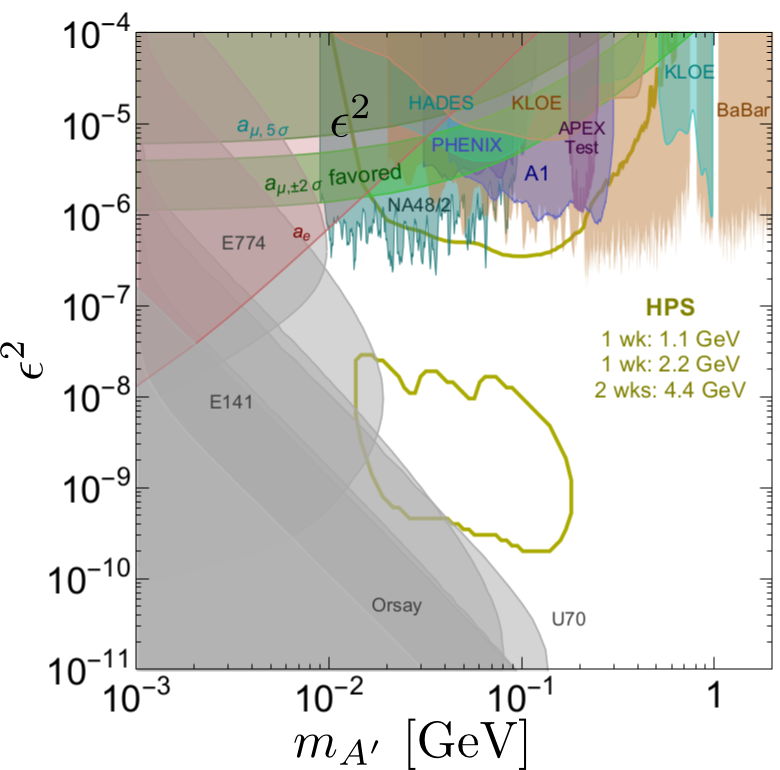
\includegraphics[width=0.9\textwidth]{images/ap_current_limits.png}
    \caption{Existing constraints on the heavy photon coupling strength.}
    \label{fig:ap_limits}
\end{figure}
